\chapter{La spectroscopie au service de la structure}\label{ch:b1:structure-spectroscopy}

Un parfumeur confie au laboratoire un liquide incolore qui sent l'ananas
et demande ce que c'est. Il y a cinquante ans, la réponse aurait demandé
des semaines de réactions de dégradation. Aujourd'hui, elle prend dix
minutes~: une analyse élémentaire donne la formule, un spectre
infrarouge nomme le groupe caractéristique, et un spectre de résonance
magnétique nucléaire du proton montre comment les atomes sont liés. Ce
chapitre explique comment se lit chaque spectre --- ce que la lumière de
chaque domaine fait à une molécule, et quels traits d'un spectre portent
quelle information de structure --- et se termine par cette molécule
d'ananas.

\begin{recall}
Le volume scolaire (années 11 et 12) a mesuré des \omterm{def:b1:structure-spectroscopy:absorbance}{absorbances} au
spectrophotomètre et utilisé la loi de Beer--Lambert pour déterminer des
concentrations, identifié des groupes caractéristiques à l'aide de tables
de bandes infrarouges, et lu des spectres simples de RMN du proton
(nombre de signaux, \omterm{def:b1:structure-spectroscopy:integration}{intégration}, règle des $n + 1$). Les liaisons
simples, doubles et triples et la liaison $\pi$ sont celles du
\cref{ch:b1:lewis-resonance-vsepr}.
\end{recall}

\section{Spectroscopie UV--visible~: conjugaison et couleur}

\begin{definition}[Absorbance et loi de Beer--Lambert]\label{def:b1:structure-spectroscopy:absorbance}
Pour une lumière d'intensité $I_0$ entrant dans une solution et
d'intensité $I$ en sortant, l'\emph{absorbance}\index{absorbance} vaut
$A = \log(I_0/I)$. Pour une solution diluée d'une seule espèce
absorbante, $A = \varepsilon\,\ell\,c$ (loi de Beer--Lambert), où $\ell$
est la longueur traversée, $c$ la concentration et $\varepsilon$ le
\emph{coefficient d'absorption
molaire}\index{coefficient d'absorption molaire}, propriété de l'espèce à
cette longueur d'onde.
\end{definition}

Une molécule absorbe la lumière ultraviolette ou visible lorsque
l'énergie d'un photon correspond à l'écart entre le plus haut niveau
électronique occupé et le plus bas niveau vide de ses liaisons. Pour les
liaisons $\sigma$, cet écart est grand et l'absorption se situe loin dans
l'ultraviolet~; les liaisons $\pi$ absorbent plus près du visible, et
une chaîne de liaisons doubles et simples alternées absorbe à des
longueurs d'onde d'autant plus grandes que la chaîne est longue.

\begin{definition}[Système conjugué, chromophore, maximum d'absorption]\label{def:b1:structure-spectroscopy:conjugation}
Un \emph{système conjugué}\index{systeme conjugue@système conjugué} est une chaîne d'atomes
portant chacun une orbitale $p$ engagée dans un système $\pi$, comme dans
une alternance de liaisons doubles et simples (buta-1,3-diène, benzène).
Le groupe d'atomes responsable d'une absorption est son
\emph{chromophore}\index{chromophore}~; la longueur d'onde à laquelle son
\omterm{def:b1:structure-spectroscopy:absorbance}{absorbance} est la plus grande est le \emph{maximum
d'absorption}\index{maximum d'absorption}, $\lambda_{\max}$.
\end{definition}

Les niveaux d'un \omterm{def:b1:structure-spectroscopy:conjugation}{système conjugué} s'étendent sur toute la chaîne et se
rapprochent à mesure que la chaîne s'allonge, comme les niveaux d'une
particule dans une boîte plus longue~: $\lambda_{\max}$ augmente avec la
conjugaison. L'éthène et le butadiène n'absorbent que dans
l'ultraviolet~; les onze liaisons doubles conjuguées du
$\beta$-carotène amènent l'absorption dans la partie bleue du visible.
Une substance prend la couleur complémentaire de la lumière qu'elle
absorbe~: absorbant le bleu et le violet, le carotène paraît orange.

\begin{omfigure}
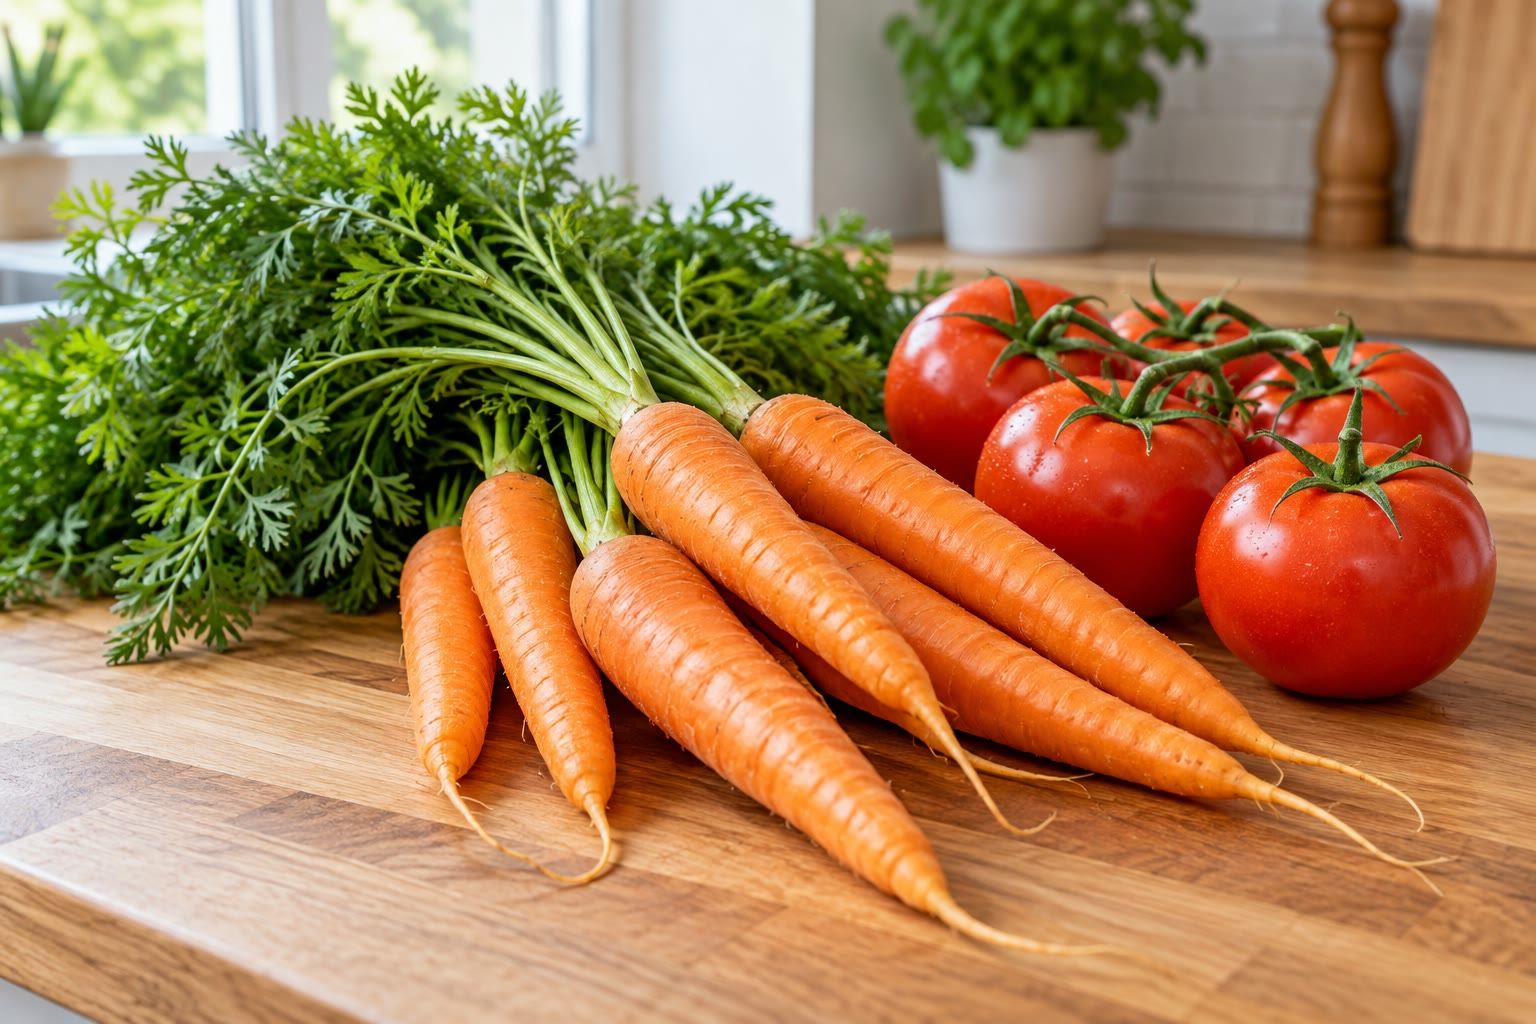
\includegraphics[width=0.55\linewidth]{images/book2/ai/b1-17-carrots-tomatoes.jpg}

{\small Les carottes et les tomates doivent leurs couleurs à de longues
molécules conjuguées, les carotènes et le lycopène, qui absorbent la
lumière bleue et verte et laissent passer l'orange et le rouge.}
\end{omfigure}

\begin{omfigure}
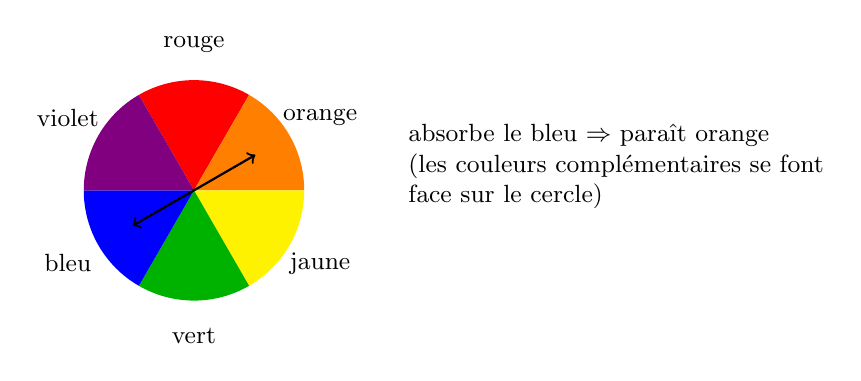
\begin{tikzpicture}[font=\small]
  \foreach \a/\c/\n in {90/red/rouge, 30/orange/orange, -30/yellow/jaune, -90/green!70!black/vert, -150/blue/bleu, 150/violet/violet} {
    \fill[\c] (0,0) -- (\a-30:1.4) arc[start angle=\a-30, end angle=\a+30, radius=1.4] -- cycle;
    \node at (\a:1.85) {\n};
  }
  \draw[<->, thick] (-150:0.9) -- (30:0.9);
  \node[align=left, anchor=west] at (2.6,0.3) {absorbe le bleu $\Rightarrow$ paraît orange\\(les couleurs complémentaires se font\\face sur le cercle)};
\end{tikzpicture}

{\small Un cercle chromatique. La couleur perçue est la complémentaire de
la couleur absorbée~: une solution qui absorbe dans le bleu paraît
orange.}
\end{omfigure}

\section{La spectroscopie infrarouge approfondie}

\begin{definition}[Nombre d'onde, transmittance, empreinte digitale]\label{def:b1:structure-spectroscopy:wavenumber}
Les spectres infrarouges sont tracés en fonction du \emph{nombre
d'onde}\index{nombre d'onde} $\tilde\nu = 1/\lambda$, en \unit{cm^{-1}},
proportionnel à l'énergie du photon. L'ordonnée est la
\emph{transmittance}\index{transmittance}
$T = I/I_0$, en pour cent, de sorte que les bandes pointent vers le bas.
En dessous de \qty{1500}{cm^{-1}} environ, de nombreuses bandes qui se
chevauchent, caractéristiques de la molécule entière plutôt que d'une
liaison, forment l'\emph{empreinte
digitale}\index{empreinte digitale} de la molécule.
\end{definition}

Une liaison absorbe la lumière infrarouge à la fréquence à laquelle
elle vibre. Comme pour deux masses reliées par un ressort, plus la
liaison est raide et plus les atomes sont légers, plus le \omterm{def:b1:structure-spectroscopy:wavenumber}{nombre d'onde}
est élevé~: les liaisons à l'hydrogène (O--H, C--H) au-dessus de
\qty{2800}{cm^{-1}}, les liaisons triples vers 2200, les liaisons
doubles vers 1700--1600, les liaisons simples entre atomes plus lourds
en dessous de 1300. Le tableau donne les positions mesurées pour les
molécules de ce chapitre, en \omterm{def:b1:extent-q-and-k:system}{phase} gazeuse, où les molécules sont
isolées.

\begin{omfigure}
\begin{tabular}{llr}
\hline
molécule & liaison & $\tilde\nu$ (\unit{cm^{-1}}) \\
\hline
éthanol & O--H & 3666 \\
éthanol & C--H & 2978 \\
éthanol & C--O & 1060 \\
propanone & C=O & 1738 \\
acide éthanoïque & O--H & 3582 \\
acide éthanoïque & C=O & 1788 \\
éthanoate d'éthyle & C=O & 1764 \\
éthanoate d'éthyle & C--O & 1238 \\
\hline
\end{tabular}

\smallskip
{\small Maxima des bandes dans des spectres infrarouges en \omterm{def:b1:extent-q-and-k:system}{phase} gazeuse.
Dans les liquides, les \omterm{def:b1:intermolecular-forces-solvents:hbond}{liaisons hydrogène} élargissent les bandes O--H et
les déplacent vers les petits \omterm{def:b1:structure-spectroscopy:wavenumber}{nombres d'onde}, et les bandes C=O des
acides descendent quand l'acide se dimérise.}
% ledger: ir:ethanol-OH, ir:ethanol-CH, ir:ethanol-CO, ir:propanone-CO, ir:ethanoic-OH, ir:ethanoic-CO, ir:ethylethanoate-CO, ir:ethylethanoate-COC
\end{omfigure}

\begin{omfigure}
\begin{tikzpicture}
\begin{axis}[name=i1, width=0.86\linewidth, height=3.2cm, xmin=500, xmax=4000, x dir=reverse, ymin=0, ymax=105, ytick={0,50,100}, ylabel={$T$ (\%)}, tick label style={font=\scriptsize}, label style={font=\small}, xticklabels={}]
\addplot[omDef, thick] table[x=nu, y=T] {figdata/out/bachelor-1-spectra-ir-ethanol.dat};
\node[font=\scriptsize, anchor=west] at (axis cs:2600,25) {éthanol};
\end{axis}
\begin{axis}[name=i2, at={(i1.south)}, anchor=north, yshift=-0.25cm, width=0.86\linewidth, height=3.2cm, xmin=500, xmax=4000, x dir=reverse, ymin=0, ymax=105, ytick={0,50,100}, ylabel={$T$ (\%)}, tick label style={font=\scriptsize}, label style={font=\small}, xticklabels={}]
\addplot[omProp, thick] table[x=nu, y=T] {figdata/out/bachelor-1-spectra-ir-propanone.dat};
\node[font=\scriptsize, anchor=west] at (axis cs:2600,25) {propanone};
\end{axis}
\begin{axis}[at={(i2.south)}, anchor=north, yshift=-0.25cm, width=0.86\linewidth, height=3.2cm, xmin=500, xmax=4000, x dir=reverse, ymin=0, ymax=105, ytick={0,50,100}, ylabel={$T$ (\%)}, tick label style={font=\scriptsize}, label style={font=\small}, xlabel={nombre d'onde (\unit{cm^{-1}})}]
\addplot[omMeth, thick] table[x=nu, y=T] {figdata/out/bachelor-1-spectra-ir-ethanoic.dat};
\node[font=\scriptsize, anchor=west] at (axis cs:2600,25) {acide éthanoïque};
\end{axis}
\end{tikzpicture}

{\small Spectres infrarouges de l'éthanol, de la propanone et de l'acide
éthanoïque, simulés à partir des positions de bandes mesurées du tableau
(hauteurs et largeurs de bandes schématiques). La bande C=O vers
\qty{1750}{cm^{-1}} et la bande O--H au-dessus de \qty{3500}{cm^{-1}}
distinguent au premier coup d'œil les trois groupes caractéristiques.}
\end{omfigure}

\section{RMN du proton~: déplacement chimique et intégration}

Dans un champ magnétique intense, un proton possède deux \omterm{def:b1:quantum-numbers:energy-level}{niveaux
d'énergie}~; des ondes radio de fréquence convenable le font passer de
l'un à l'autre. Cette fréquence est proportionnelle au champ magnétique
que ressent réellement le proton, que les électrons qui l'entourent
réduisent légèrement. Des protons situés dans des environnements
chimiques différents résonnent donc à des fréquences légèrement
différentes.

\begin{definition}[Déplacement chimique, blindage, protons équivalents]\label{def:b1:structure-spectroscopy:chemical-shift}
Le \emph{déplacement chimique}\index{deplacement chimique@déplacement chimique} d'un proton vaut
$\delta = (\nu - \nu_{\text{réf}})/\nu_0 \times 10^6$, en \unit{ppm}, où
$\nu$ est sa fréquence de résonance, $\nu_{\text{réf}}$ celle des
protons du tétraméthylsilane et $\nu_0$ la fréquence de fonctionnement
du spectromètre. La diminution du champ ressenti par un noyau, due à ses
électrons, est son \emph{blindage}\index{blindage}~: des voisins
électroattracteurs (O, halogènes, C=O) déblindent un proton et
augmentent son $\delta$. Des \emph{protons équivalents}\index{protons equivalents@protons équivalents} sont des
protons échangés par une symétrie de la molécule ou par une rotation
rapide~; ils ont le même déplacement chimique.
\end{definition}

\begin{proposition}[Le déplacement ne dépend pas du spectromètre]\label{prop:b1:structure-spectroscopy:shift-field-independent}
Le \omterm{def:b1:structure-spectroscopy:chemical-shift}{déplacement chimique} d'un proton est le même sur des spectromètres de
champs différents.
\end{proposition}

\begin{proof}
$\nu$ et $\nu_{\text{réf}}$ sont tous deux proportionnels au champ
appliqué $B_0$ (chacun multiplié par son propre facteur de \omterm{def:b1:structure-spectroscopy:chemical-shift}{blindage}), et
$\nu_0$ l'est aussi. Le rapport $(\nu - \nu_{\text{réf}})/\nu_0$ est donc
indépendant de $B_0$. Les écarts en hertz, au contraire, augmentent avec
le champ.
\end{proof}

\begin{definition}[Intégration]\label{def:b1:structure-spectroscopy:integration}
L'\emph{intégration}\index{integration@intégration} d'un signal est son aire, lue sur le
spectre comme la hauteur d'une courbe en marches~; les aires sont
proportionnelles aux nombres de protons qui donnent les signaux.
\end{definition}

\section{Le couplage spin--spin}

\begin{definition}[Couplage spin--spin, constante de couplage, multiplet]\label{def:b1:structure-spectroscopy:coupling}
À travers les liaisons, l'état magnétique d'un proton modifie légèrement
le champ ressenti par les protons des carbones voisins~: ce
\emph{couplage spin--spin}\index{couplage spin--spin} scinde chaque
signal en un \emph{multiplet}\index{multiplet} de raies séparées par la
\emph{constante de couplage}\index{constante de couplage} $J$, en hertz.
Deux protons couplés entre eux présentent le même $J$~; des \omterm{def:b1:structure-spectroscopy:chemical-shift}{protons
équivalents} ne se scindent pas mutuellement leur signal.
\end{definition}

\begin{proposition}[La règle des \texorpdfstring{$n + 1$}{n + 1}]\label{prop:b1:structure-spectroscopy:n-plus-one}
Un proton (ou un ensemble de \omterm{def:b1:structure-spectroscopy:chemical-shift}{protons équivalents}) couplé avec la même
constante $J$ à $n$ voisins équivalents donne $n + 1$ raies, séparées de
$J$, d'intensités relatives égales aux coefficients binomiaux
$\binom{n}{k}$, $k = 0$ à $n$ (\emph{règle des $n + 1$}\index{regle des n + 1@règle des $n + 1$}).
\end{proposition}

\begin{proof}
Chaque voisin est dans l'un de deux états de spin, qui décale la raie
observée de $+J/2$ ou de $-J/2$. Avec $n$ voisins, le décalage vaut
$(k - n/2)J$, où $k$ est le nombre de voisins dans le premier état~:
$n + 1$ valeurs, régulièrement espacées de $J$. Les deux états étant
presque également peuplés, les $2^n$ combinaisons sont équiprobables, et
$k$ voisins dans le premier état se réalisent de $\binom{n}{k}$ façons.
\end{proof}

\begin{omfigure}
\begin{tikzpicture}[font=\small, x=0.85cm, y=0.5cm]
  % quartet: three neighbours, each split +-J/2 (J = 1.5 units)
  \draw[thick] (0,4) -- (0,3.4);
  \foreach \x in {-0.75,0.75} \draw (0,3.4) -- (\x,2.4);
  \foreach \a/\b in {-0.75/-1.5, -0.75/0, 0.75/0, 0.75/1.5} \draw (\a,2.4) -- (\b,1.4);
  \foreach \a/\b in {-1.5/-2.25, -1.5/-0.75, 0/-0.75, 0/0.75, 1.5/0.75, 1.5/2.25} \draw (\a,1.4) -- (\b,0.4);
  \foreach \x/\h in {-2.25/1, -0.75/3, 0.75/3, 2.25/1} {\draw[omDef, very thick] (\x,-2.6) -- (\x,{-2.6+0.7*\h}); \draw[dotted] (\x,0.4) -- (\x,{-2.6+0.7*\h});}
  \draw (-2.8,-2.6) -- (2.8,-2.6);
  \node at (0,-3.4) {quadruplet 1\,:\,3\,:\,3\,:\,1 (\ce{-CH2-} voisin de \ce{-CH3})};
  % triplet: two neighbours
  \begin{scope}[xshift=7.5cm]
  \draw[thick] (0,4) -- (0,3.4);
  \foreach \x in {-0.75,0.75} \draw (0,3.4) -- (\x,2.4);
  \foreach \a/\b in {-0.75/-1.5, -0.75/0, 0.75/0, 0.75/1.5} \draw (\a,2.4) -- (\b,1.4);
  \foreach \x/\h in {-1.5/1, 0/2, 1.5/1} {\draw[omProp, very thick] (\x,-2.6) -- (\x,{-2.6+0.7*\h}); \draw[dotted] (\x,1.4) -- (\x,{-2.6+0.7*\h});}
  \draw (-2.1,-2.6) -- (2.1,-2.6);
  \draw[<->] (-1.5,-0.6) -- (0,-0.6) node[midway, above, font=\scriptsize] {$J$};
  \node at (0,-3.4) {triplet 1\,:\,2\,:\,1 (\ce{-CH3} voisin de \ce{-CH2-})};
  \end{scope}
\end{tikzpicture}

{\small Arbres de couplage. Chaque voisin scinde chaque raie en deux, à
$J$ l'une de l'autre~; les raies qui coïncident s'additionnent, ce qui
donne les intensités binomiales.}
\end{omfigure}

\begin{omfigure}
\begin{tikzpicture}
\begin{axis}[name=ea,
  width=0.86\linewidth, height=4.2cm, xmin=0.8, xmax=4.5, x dir=reverse, ymin=0, ymax=1.15,
  axis x line=bottom, axis y line=none, xlabel={$\delta$ (ppm)},
  tick label style={font=\scriptsize}, label style={font=\small}]
\addplot[omDef, thin] table[x=ppm, y=I] {figdata/out/bachelor-1-spectra-nmr-ethylethanoate.dat};
\node[font=\scriptsize, anchor=south] at (axis cs:4.12,0.75) {q, 2H};
\node[font=\scriptsize, anchor=west] at (axis cs:2.0,0.95) {s, 3H};
\node[font=\scriptsize, anchor=west] at (axis cs:1.15,0.8) {t, 3H};
\node[font=\small, anchor=north] at (axis cs:3.0,1.1) {\ce{CH3COOCH2CH3}};
\end{axis}
\begin{axis}[at={(ea.south)}, anchor=north, yshift=-1.3cm,
  width=0.86\linewidth, height=4.2cm, xmin=0.8, xmax=4.5, x dir=reverse, ymin=0, ymax=1.15,
  axis x line=bottom, axis y line=none, xlabel={$\delta$ (ppm)},
  tick label style={font=\scriptsize}, label style={font=\small}]
\addplot[omProp, thin] table[x=ppm, y=I] {figdata/out/bachelor-1-spectra-nmr-ethanol.dat};
\node[font=\scriptsize, anchor=south] at (axis cs:3.69,0.75) {q, 2H};
\node[font=\scriptsize, anchor=west] at (axis cs:2.55,0.6) {s, 1H};
\node[font=\scriptsize, anchor=west] at (axis cs:1.1,0.8) {t, 3H};
\node[font=\small, anchor=north] at (axis cs:2.9,1.1) {\ce{CH3CH2OH}};
\end{axis}
\end{tikzpicture}

{\small Spectres de RMN du proton de l'éthanoate d'éthyle (en haut) et de
l'éthanol (en bas) dans \ce{CDCl3}, simulés à \qty{90}{MHz} à partir de
déplacements et de \omterm{def:b1:structure-spectroscopy:coupling}{constantes de couplage} mesurés
($J = \qty{7.2}{Hz}$ et \qty{7.0}{Hz}). Le quadruplet \ce{OCH2} est
déblindé par l'oxygène~; dans l'éthanol, le proton de OH, échangé
rapidement entre molécules, ne se couple pas et son déplacement dépend
de la concentration.}
% ledger: nmr:ethylethanoate-OCH2, nmr:ethylethanoate-COCH3, nmr:ethylethanoate-CH3, nmr:ethylethanoate-J, nmr:ethanol-CH2, nmr:ethanol-CH3, nmr:ethanol-OH, nmr:ethanol-J
\end{omfigure}

\begin{omfigure}
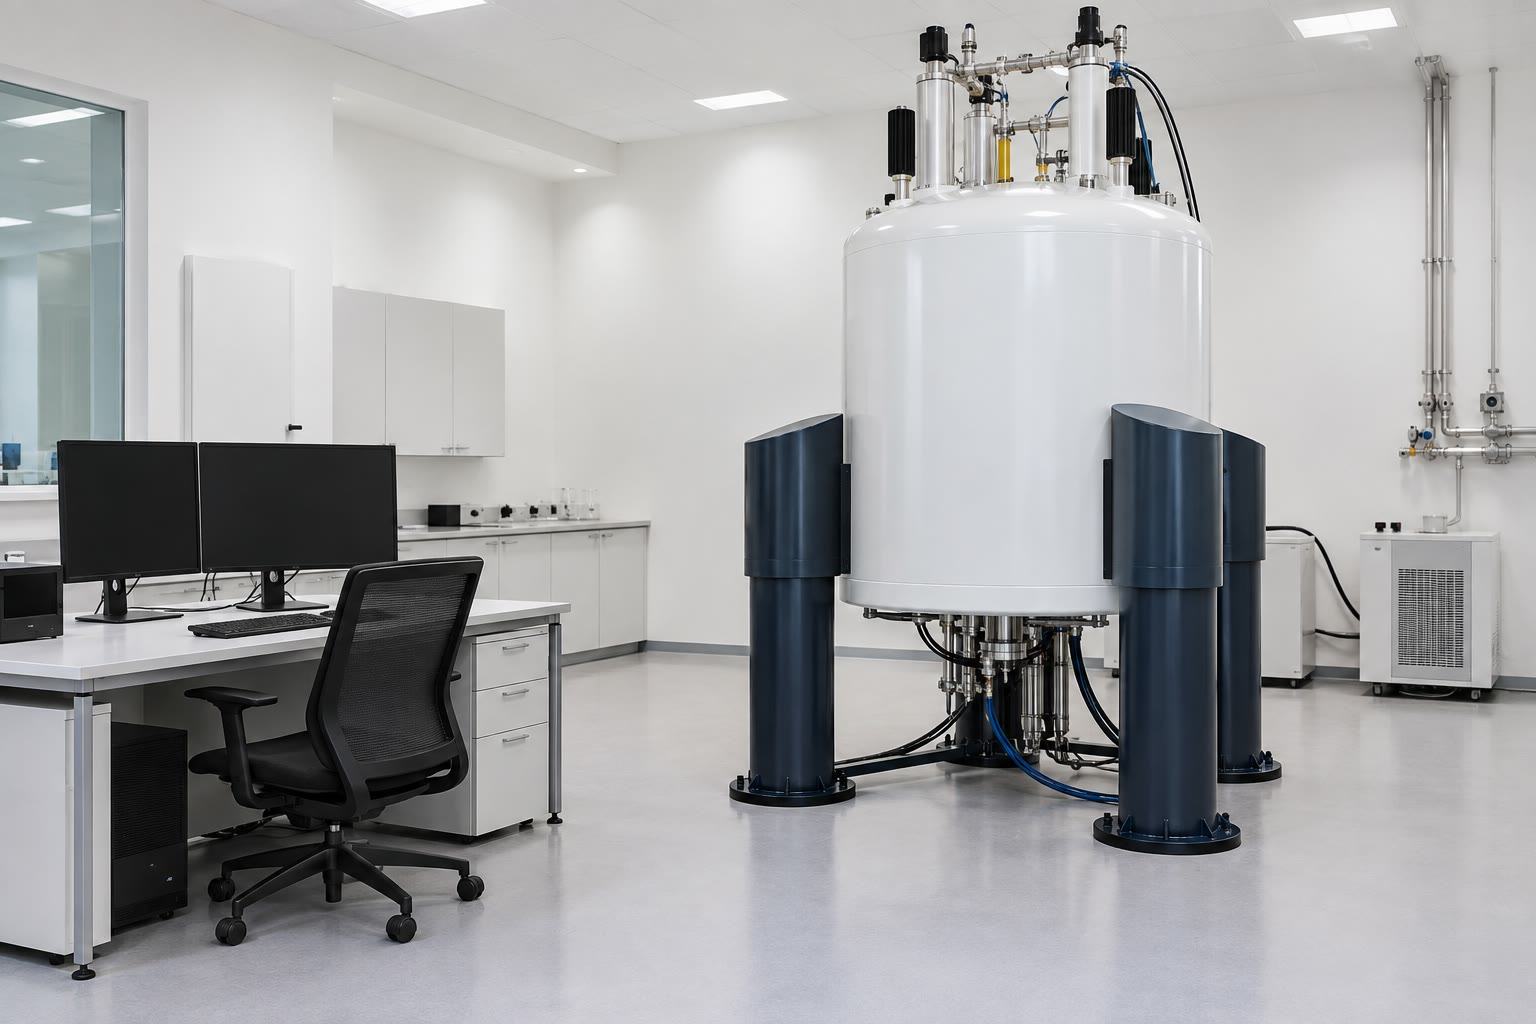
\includegraphics[width=0.5\linewidth]{images/book2/ai/b1-17-nmr.jpg}

{\small Un spectromètre de RMN~: le grand cylindre contient un aimant
supraconducteur refroidi à l'hélium liquide~; le tube d'échantillon est
descendu en son centre.}
\end{omfigure}

\section{Résoudre une structure}

\begin{definition}[Nombre d'insaturations]\label{def:b1:structure-spectroscopy:unsaturation}
Le \emph{nombre d'insaturations}\index{nombre d'insaturations} d'une
formule est le nombre de cycles augmenté du nombre de liaisons $\pi$ de
la molécule.
\end{definition}

\begin{proposition}[Nombre d'insaturations à partir de la formule]\label{prop:b1:structure-spectroscopy:unsaturation-formula}
Pour une molécule $\mathrm{C}_c\mathrm{H}_h\mathrm{N}_n\mathrm{O}_o\mathrm{X}_x$
(X un halogène), le \omterm{def:b1:structure-spectroscopy:unsaturation}{nombre d'insaturations} vaut
\[
  D = \frac{2c + 2 + n - h - x}{2} .
\]
\end{proposition}

\begin{proof}
Une chaîne ouverte de $c$ carbones ne comportant que des liaisons simples
porte $2c + 2$ hydrogènes. Chaque cycle ou liaison $\pi$ en retire deux.
Un oxygène divalent inséré dans une chaîne ne change rien~; un azote
trivalent apporte un hydrogène de plus~; un halogène prend la place d'un
hydrogène. Compter les hydrogènes manquants et diviser par deux donne
$D$.
\end{proof}

\begin{method}[Résoudre une structure]\label{met:b1:structure-spectroscopy:solve-structure}
\begin{enumerate}
  \item À partir de la formule, calculer $D$.
  \item À partir du spectre IR, repérer les groupes caractéristiques
        (C=O, O--H, N--H, C--O) et l'absence des autres.
  \item À partir du spectre de RMN~: nombre de signaux (ensembles de
        \omterm{def:b1:structure-spectroscopy:chemical-shift}{protons équivalents}), \omterm{def:b1:structure-spectroscopy:integration}{intégrations} (protons par ensemble),
        \omterm{def:b1:structure-spectroscopy:chemical-shift}{déplacements chimiques} (groupes voisins), multiplicités des
        signaux (nombre de voisins d'après la règle des $n + 1$),
        \omterm{def:b1:structure-spectroscopy:coupling}{constantes de couplage} (quels signaux sont voisins).
  \item Construire des fragments, les assembler, et confronter chaque
        pic à la structure proposée~; écarter les isomères qui ne
        conviennent pas.
\end{enumerate}
\end{method}

\section{Exercices}

\begin{exercise}[$\star$]\label{exo:b1:structure-spectroscopy:1}
Une solution d'un colorant à \qty{2.0e-5}{mol/L} dans une cuve de
\qty{1.00}{cm} a une \omterm{def:b1:structure-spectroscopy:absorbance}{absorbance} de 0.64 à son \omterm{def:b1:structure-spectroscopy:conjugation}{maximum d'absorption}.
Calculer $\varepsilon$, ainsi que l'\omterm{def:b1:structure-spectroscopy:absorbance}{absorbance} d'une solution trois fois
plus concentrée.
\end{exercise}

\begin{exercise}[$\star$]\label{exo:b1:structure-spectroscopy:2}
Calculer le \omterm{def:b1:structure-spectroscopy:unsaturation}{nombre d'insaturations} de \ce{C6H6}, \ce{C4H8O2},
\ce{C3H7NO}, \ce{C2H3Cl} et \ce{C10H14O} (la carvone). Proposer une
structure pour chacun.
\end{exercise}

\begin{exercise}[$\star$]\label{exo:b1:structure-spectroscopy:3}
Combien de signaux de protons, et avec quelles \omterm{def:b1:structure-spectroscopy:integration}{intégrations}, donnent la
propanone, l'acide éthanoïque, le 2-méthylpropane et le
1,2-dichloroéthane~?
\end{exercise}

\begin{exercise}[$\star$]\label{exo:b1:structure-spectroscopy:4}
Un signal se trouve à \qty{1460}{Hz} du tétraméthylsilane sur un
spectromètre à \qty{400}{MHz}. Quel est son \omterm{def:b1:structure-spectroscopy:chemical-shift}{déplacement chimique}~? À
combien de hertz se trouverait-il à \qty{90}{MHz}~? Pourquoi les champs
intenses séparent-ils mieux les \omterm{def:b1:structure-spectroscopy:coupling}{multiplets}~?
\end{exercise}

\begin{exercise}[$\star\star$]\label{exo:b1:structure-spectroscopy:5}
Prévoir la multiplicité de chaque signal du 1-bromopropane,
\ce{CH3CH2CH2Br}, en supposant les \omterm{def:b1:structure-spectroscopy:coupling}{constantes de couplage} égales, ainsi
que les intensités relatives des raies du signal central.
\end{exercise}

\begin{exercise}[$\star\star$]\label{exo:b1:structure-spectroscopy:6}
En quoi les spectres IR de l'éthanol, de la propanone et de l'acide
éthanoïque diffèrent-ils entre 1700 et \qty{3700}{cm^{-1}}~? Quel
composé donne à la fois une bande C=O et une bande O--H~?
\end{exercise}

\begin{exercise}[$\star\star$]\label{exo:b1:structure-spectroscopy:7}
Deux isomères \ce{C4H8O2}~: l'éthanoate d'éthyle et le propanoate de
méthyle. Prévoir leurs spectres de RMN (déplacements approximatifs,
multiplicités, \omterm{def:b1:structure-spectroscopy:integration}{intégrations}) et dire comment les distinguer.
\end{exercise}

\begin{exercise}[$\star\star$]\label{exo:b1:structure-spectroscopy:8}
À partir du spectre simulé de l'éthanoate d'éthyle, lire l'écart entre
deux raies du quadruplet en ppm et le convertir en hertz (le spectre est
simulé à \qty{90}{MHz}). Comparer avec le triplet.
\end{exercise}

\begin{exercise}[$\star\star$]\label{exo:b1:structure-spectroscopy:9}
Un composé \ce{C3H6O} présente une bande IR intense à
\qty{1738}{cm^{-1}} et un seul signal de RMN. L'identifier. Quel isomère
présenterait une bande vers \qty{2720}{cm^{-1}} et un signal vers
\qty{9.8}{ppm}~?
\end{exercise}

\begin{exercise}[$\star\star\star$]\label{exo:b1:structure-spectroscopy:10}
Démontrer la règle des $n + 1$ sous la forme suivante~: un proton couplé
à deux ensembles différents de voisins, $n_1$ avec $J_1$ et $n_2$ avec
$J_2$, donne $(n_1 +
1)(n_2 + 1)$ raies. Lorsque $J_1 = J_2$, combien reste-t-il de raies
distinctes~? Appliquer au \ce{CH2} central du 1-bromopropane.
\end{exercise}

\begin{exercise}[$\star\star\star$]\label{exo:b1:structure-spectroscopy:11}
Un composé \ce{C4H10O} ne donne aucune bande IR entre 1700 et 1800 mais
une large bande vers \qty{3350}{cm^{-1}} à l'état liquide, et un spectre
de RMN comportant un doublet (6H), un \omterm{def:b1:structure-spectroscopy:coupling}{multiplet} (1H), un doublet (2H) et
un singulet élargi (1H). Trouver la structure.
\end{exercise}

\begin{exercise}[$\star\star\star$]\label{exo:b1:structure-spectroscopy:12}
Montrer que l'\omterm{def:b1:structure-spectroscopy:absorbance}{absorbance} d'un mélange de deux espèces vérifie $A = \ell(\varepsilon_1c_1
+ \varepsilon_2c_2)$, et expliquer comment des mesures à deux longueurs
d'onde donnent les deux concentrations.
\end{exercise}

\section{Problème~: la molécule d'ananas}

\begin{problem}[{Problème du week-end --- analyse par combustion et
densité de vapeur, spectre infrarouge, spectre de RMN du proton, et
structure et masse molaire de l'ester à odeur d'ananas}]
\label{pb:b1:structure-spectroscopy:1}
L'inconnu est un liquide qui ne contient que C, H et O. La combustion de
\qty{0.2500}{g} donne \qty{0.5690}{g} de dioxyde de carbone et
\qty{0.2328}{g} d'eau. Sa vapeur a une masse volumique de
\qty{3.74}{g/L} à
\qty{100}{\celsius} et sous \qty{1.000}{bar}. Bandes IR en \omterm{def:b1:extent-q-and-k:system}{phase}
gazeuse~: 2982,
1754, \qty{1182}{cm^{-1}} (intense), aucune au-dessus de
\qty{3100}{cm^{-1}}. RMN du proton (\ce{CDCl3})~: 4.13 (q, 2H, $J = \qty{7.2}{Hz}$),
2.28 (t, 2H), 1.66 (sextuplet, 2H), 1.25 (t, 3H, $J = \qty{7.2}{Hz}$), 0.95
(t, 3H) ppm. $M$~: C 12.0, H 1.0, O \qty{16.0}{g/mol}~; $R =
\qty{8.314}{J/(K.mol)}$.
% ledger: ir:ethylbutanoate-CH, ir:ethylbutanoate-CO, ir:ethylbutanoate-COC, nmr:ethylbutanoate-OCH2, nmr:ethylbutanoate-CH2CO, nmr:ethylbutanoate-CH2, nmr:ethylbutanoate-OCH2CH3, nmr:ethylbutanoate-CH3, nmr:ethylbutanoate-J

\begin{center}
\begin{tikzpicture}
\begin{axis}[width=0.86\linewidth, height=4.0cm, xmin=0.6, xmax=4.5, x dir=reverse, ymin=0, ymax=1.15,
  axis x line=bottom, axis y line=none, xlabel={$\delta$ (ppm)},
  tick label style={font=\scriptsize}, label style={font=\small}]
\addplot[omDef, thin] table[x=ppm, y=I] {figdata/out/bachelor-1-spectra-nmr-ethylbutanoate.dat};
\end{axis}
\end{tikzpicture}
\end{center}

\medskip
\noindent\textbf{Partie I --- La formule.}
\begin{enumerate}
  \item Calculer la masse de carbone de l'échantillon.
  \item Calculer la masse d'hydrogène.
  \item En déduire la masse d'oxygène.
  \item Calculer les pourcentages massiques de C, H et O.
  \item Trouver la formule empirique.
  \item À partir de la masse volumique de la vapeur, calculer la masse
        molaire (gaz parfait).
  \item Donner la formule brute et son \omterm{def:b1:structure-spectroscopy:unsaturation}{nombre d'insaturations}.
\end{enumerate}

\medskip
\noindent\textbf{Partie II --- Le spectre infrarouge.}
\begin{enumerate}[resume]
  \item Attribuer la bande à \qty{1754}{cm^{-1}}.
  \item Qu'exclut l'absence de bandes au-dessus de \qty{3100}{cm^{-1}}~?
  \item Attribuer la bande intense à \qty{1182}{cm^{-1}}.
  \item Attribuer la bande à \qty{2982}{cm^{-1}}.
  \item Compte tenu du \omterm{def:b1:structure-spectroscopy:unsaturation}{nombre d'insaturations}, quelle famille de
        composés reste-t-il~? Pourquoi pas un acide carboxylique, une
        cétone portant un groupe éther, ou un diol cyclique~?
\end{enumerate}

\medskip
\noindent\textbf{Partie III --- Le spectre de RMN.}
\begin{enumerate}[resume]
  \item Combien d'ensembles de \omterm{def:b1:structure-spectroscopy:chemical-shift}{protons équivalents}~? Vérifier
        l'\omterm{def:b1:structure-spectroscopy:integration}{intégration} totale.
  \item Interpréter le quadruplet à 4.13 ppm~: voisins et environnement.
  \item Interpréter le triplet à 1.25 ppm. Pourquoi les deux signaux
        ont-ils le même $J$~?
  \item Interpréter le triplet à 2.28 ppm.
  \item Interpréter le sextuplet à 1.66 ppm.
  \item Interpréter le triplet à 0.95 ppm.
  \item Construire les deux fragments que décrivent ces signaux.
  \item Pourquoi les signaux à 4.13 et 2.28 ppm sont-ils les plus
        déblindés~?
\end{enumerate}

\medskip
\noindent\textbf{Partie IV --- La structure.}
\begin{enumerate}[resume]
  \item Assembler les fragments par le groupe ester~: deux possibilités.
        Laquelle est cohérente avec les \omterm{def:b1:structure-spectroscopy:chemical-shift}{déplacements chimiques}~?
  \item Expliquer pourquoi le propanoate de propyle ne convient pas.
  \item Expliquer pourquoi l'éthanoate de butyle ne convient pas.
  \item Nommer le composé et dessiner sa structure.
  \item Confronter chaque bande IR et chaque signal de RMN à la structure.
  \item Donner la masse molaire de la molécule d'ananas.
\end{enumerate}
\end{problem}
